% 简洁风格：浅色背景 + 细边框 + 行号 + 自动换行
\definecolor{codebg}{RGB}{248,249,250}
\definecolor{codeframe}{RGB}{220,223,228}
\definecolor{codekw}{RGB}{25,85,145}
\definecolor{codecm}{RGB}{90,125,90}
\definecolor{codestr}{RGB}{136,44,136}

\lstdefinestyle{cleancpp}{
	language=C++,
	basicstyle=\ttfamily\small,
	keywordstyle=\bfseries\color{codekw},
    commentstyle=\color{codecm},
	stringstyle=\color{codestr},
	backgroundcolor=\color{codebg},
	frame=single,
	rulecolor=\color{codeframe},
	framesep=6pt,
	numbers=left,
	numberstyle=\scriptsize\color{gray},
	numbersep=8pt,
	breaklines=true,
	breakatwhitespace=false,
	showstringspaces=false,
	keepspaces=true,
	tabsize=4,
	columns=fullflexible
}

\chapter{Exercise 1.1}

\section{Problem}

\begin{enumerate}
    \item Imagine an artificial computer language, which can be utilized to solve a practical problem, i.e. the application of the language.
    \begin{itemize}
        \item Tips 1. Language is an alternative approach to problem solving.
        \item Tips 2. First find a proper problem, then design a language to solve the problem.
    \end{itemize}
    \item Give an example of a complete piece written in the proposed language.
    \item Discuss how to define the new language and try your approach.
    \item Describe the process of changing the thinking of your language to a reality, i.e. how to make the artificial language usable.
\end{enumerate}

\section{Solution}

\subsection{Problem 1}

\textbf{Background:} The "Chaos" of University Life

University students face conflicting fixed courses, flexible tasks, and resource constraints. Generic calendars lack logic for dependencies and auto-scheduling.

\textbf{My solution}: A Declarative Scheduling DSL

Instead of manually dragging blocks on a calendar, I propose \textbf{UniPlan}, a Domain-Specific Language (DSL) designed specifically for academic life.

Key Features:
\begin{itemize}
    \item Dependency Awareness: Explicitly define logical links (e.g., Task B requires Task A to be completed).
    \item Resource Tagging: Tasks can tag required environments (Library, Lab, Online), preventing impossible schedules.
    \item Elasticity: Tasks can be marked as splittable (can be broken into chunks) or atomic (must be done in one go).
    \item Priority-Driven Optimization: The compiler uses a greedy or constraint-solving algorithm to fit high-priority tasks first, pushing lower-priority ones to remaining slots or flagging conflicts.
\end{itemize}


\subsection{Problem 2}

Here is an example of UniPlan code for a student’s week plan:

\begin{lstlisting}[style=cleancpp]
// --- 1. Resource Definitions ---
Environment Lab { location: "CS_Building_Room302"; noise_level: High; }
Environment Library { location: "Main_Library_Floor2"; noise_level: Low; }

// --- 2. Fixed Constraints (Immutable) ---
Course Compiler_Theory {
    day: Monday;
    start: 08:00; end: 09:40;
    location: "Classroom_A101";
    type: Fixed;
}

Course Data_Lab {
    day: Wednesday;
    start: 14:00; end: 16:00;
    location: Lab;
    type: Fixed;
}

// --- 3. Flexible Tasks (To be Scheduled) ---
Task Midterm_Review {
    subject: "Compiler Theory";
    duration: 3 hours;
    deadline: Friday 18:00;
    environment: Library;       // Requires quiet zone
    priority: Critical;         // Highest priority
    splittable: false;          // Must be done in one focus block
}

Task Lab_Report {
    subject: "Data Structures";
    duration: 2 hours;
    deadline: Thursday 23:59;
    depends_on: Data_Lab;       // LOGIC: Can only start after the lab ends
    environment: Any;
    priority: High;
    splittable: true;           // Can be split into 1h + 1h
}

Task Club_Meeting {
    subject: "Robotics Club";
    duration: 1 hour;
    time_window: Tuesday 18:00 - 21:00; // Flexible within this window
    priority: Low;
}

// --- 4. Global Schedule Configuration ---
Schedule Week_Midterm {
    start_day: Monday;
    active_hours: 08:00 - 22:00;
    break_policy: 15min per 2hours;
    
    // Command the compiler to solve the puzzle
    auto_schedule: [Midterm_Review, Lab_Report, Club_Meeting];
    
    // Output format
    export_to: "google_calendar.ics";
}
\end{lstlisting}

\subsection{Problem 3}

To rigorously define UniPlan, we must move from informal ideas to formal mathematical specifications. My approach follows the standard compiler design methodology: defining the Alphabet (what characters are allowed) and the Syntactic Structure (how those characters form valid sentences).

\textbf{Alphabet}:
\begin{itemize}
    \item Letters: a-z, A-Z(Used for keywords like Task, Course and identifiers)
    \item Digits: 0-9 (Used for time, duration, priority levels)
    \item Symbols: \{ \} : ; [ ] \_ (Used for structuring the code)
\end{itemize}

\textbf{Syntax Definition (BFN)}:

\begin{lstlisting}[style=cleancpp]
<program>       ::= <definition_list> <schedule_block>

<definition_list> ::= <definition> | <definition> <definition_list>

<definition>    ::= <course_def> | <task_def> | <env_def>

// 1. Course Definition (Fixed Time)
<course_def>    ::= "Course" <identifier> "{" <course_prop_list> "}"

<course_prop_list> ::= <course_prop> | <course_prop> ";" <course_prop_list>
<course_prop>   ::= "day" ":" <day_literal>
                  | "start" ":" <time_literal>
                  | "end" ":" <time_literal>
                  | "location" ":" <string>

// 2. Task Definition (Flexible)
<task_def>      ::= "Task" <identifier> "{" <task_prop_list> "}"

<task_prop_list> ::= <task_prop> | <task_prop> ";" <task_prop_list>
<task_prop>     ::= "duration" ":" <number> "hours"
                  | "deadline" ":" <day_literal> <time_literal>
                  | "depends_on" ":" <identifier>
                  | "priority" ":" <priority_level>
                  | "splittable" ":" ("true" | "false")

<priority_level>::= "Low" | "Medium" | "High" | "Critical"

// 3. Schedule Block (The Solver Trigger)
<schedule_block>::= "Schedule" <identifier> "{" <sched_prop_list> "}"

<sched_prop_list>::= <sched_prop> | <sched_prop> ";" <sched_prop_list>
<sched_prop>    ::= "auto_schedule" ":" "[" <id_list> "]"
                  | "active_hours" ":" <time_literal> "-" <time_literal>
                  | "export_to" ":" <string>

<id_list>       ::= <identifier> | <identifier> "," <id_list>

// Terminals
<identifier>    ::= <letter> { <letter> | <digit> | "_" }
<day_literal>   ::= "Mon" | "Tue" | "Wed" | "Thu" | "Fri" | "Sat" | "Sun"
<time_literal>  ::= <digit> <digit> ":" <digit> <digit>
<string>        ::= "\"" { <any_char_except_quote> } "\""
<number>        ::= <digit> { <digit> }
\end{lstlisting}

In order to make the language understandable, I separates Course (rigid) from Task (flexible), reflecting the real-world distinction between fixed classes and homework.

\subsection{Problem 4}

Transform abstract text into a concrete .ics calendar file through a \textbf{5-stage pipeline}.

\begin{enumerate}
    \item \textbf{Lexical Analysis}: Scans raw text, discards whitespace, and outputs a stream of Tokens (keywords, IDs, numbers).
    \item \textbf{Syntax Analysis}: Parses tokens against BNF rules to build a hierarchical Abstract Syntax Tree (AST).
    \item \textbf{Semantic Analysis}: Validates logic (dependencies, time conflicts) and builds a Constraint Model.
    \item \textbf{Solver Execution}: Algorithms (e.g., Backtracking/Z3) compute optimal time slots, splitting tasks to fit gaps.
    \item \textbf{Code Generation}: Translates the solved schedule into a standard format of file for immediate import into Google/Outlook Calendar.
\end{enumerate}

\chapter{Exercise 1.2}

\section{Problem}

\begin{enumerate}
    \item Draw a T-diagram with two stages of bootstrappings.
        \begin{itemize}
            \item Given a new programming language L++, we firstly implement L, a small subset of L++.
            \item Then we use L to implement L+, a subset of L++ and a superset of L.
            \item Finally, L++ is implemented using L+.
        \end{itemize}
\end{enumerate}

\section{Solution}

\begin{figure}[htbp]
    \centering
    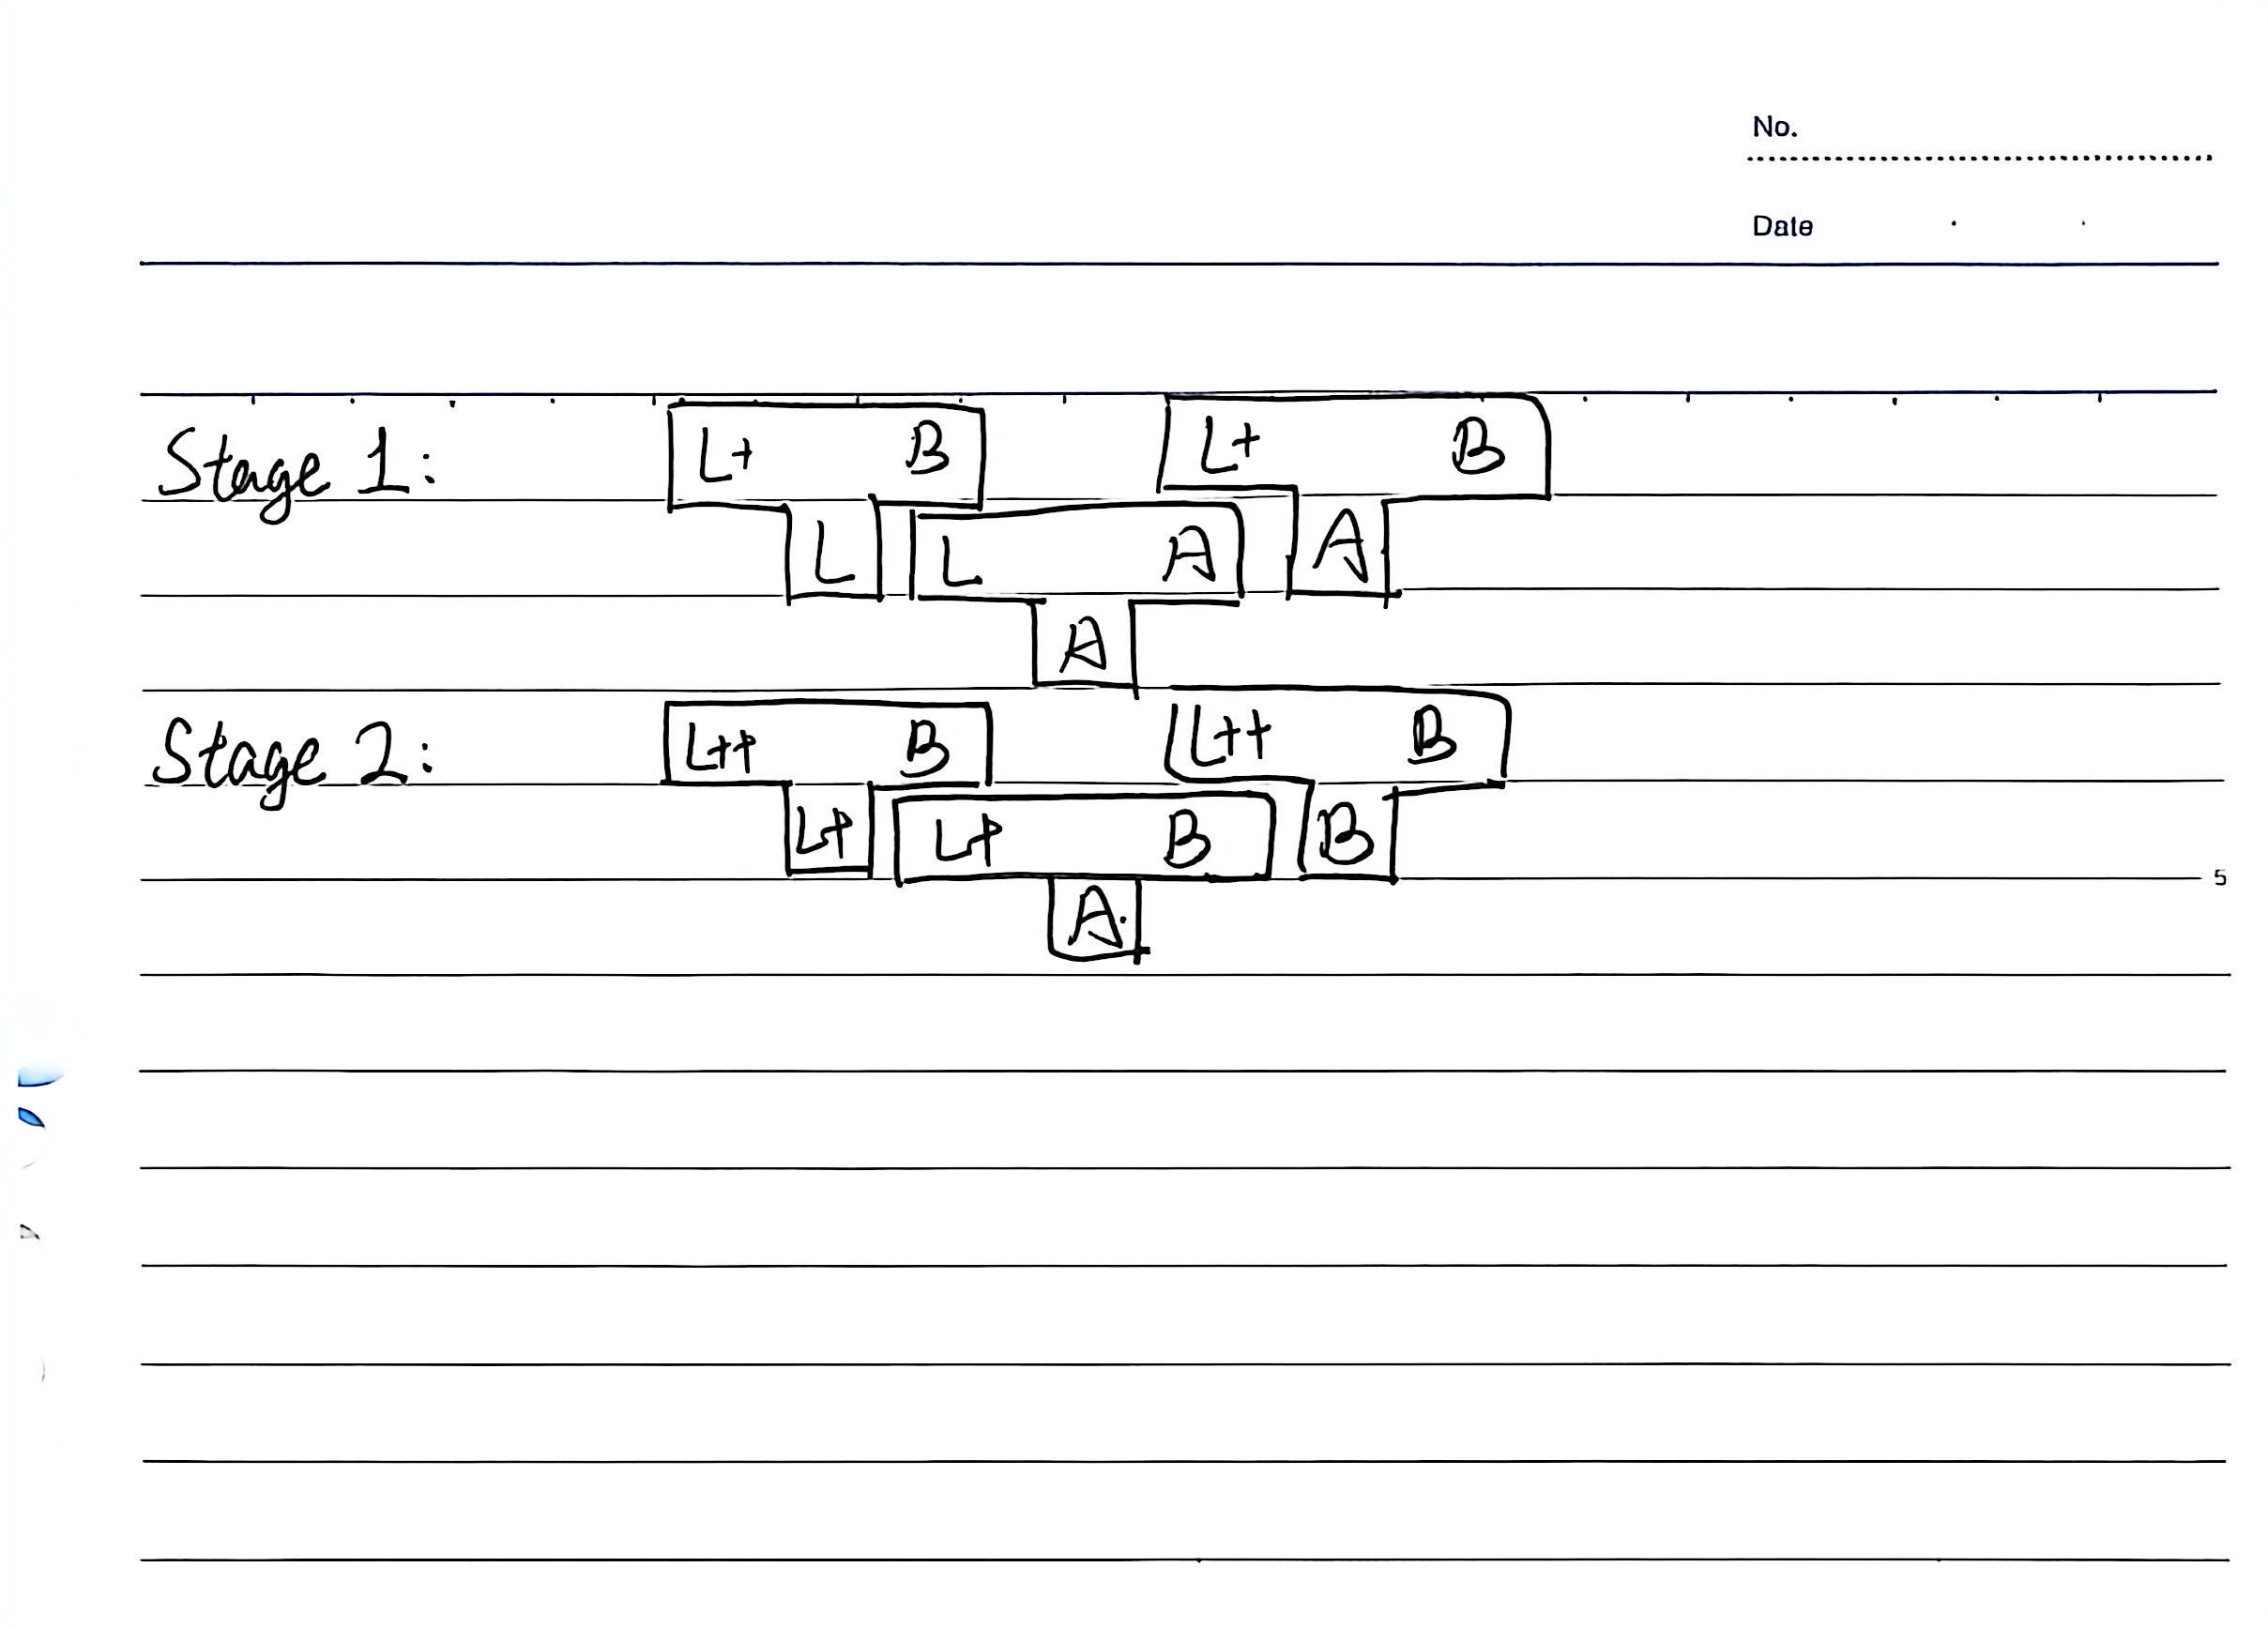
\includegraphics[width=\textwidth]{image/exercise1_1.JPG}
\end{figure}
